\documentclass[a4paper]{report}

\newtheorem{defi}{Definition}
\newtheorem{proof}{Proof}

\usepackage{graphicx}
\usepackage[T1]{fontenc}


\begin{document}

\title{Study On NP-complete problems}
\author{Adam Jama}

\maketitle

\pagenumbering{roman}

\chapter{Definition Of 8 Problems}

\subsection{Graph Colouring}
\begin{defi}
In graph computational theory the graph colouring problem is a special assignment of which is traditionally assigned with colours. In the more common approach of the graph colouring problem is a way of colouring the vertices of an undirected graph such that no two adjacent vertices share the same colour.
\end{defi}

There are two fundamental steps with the graph colouring process. The first is the decision process which we input a graph $\emph{G}$ with $\emph{n}$ vertices and choose an integer $\emph{K}$ where the graph colouring problem decision in yes. The example of the first case where the decision would be NP-complete would be the 3 colouring as shown below.



\begin{center}
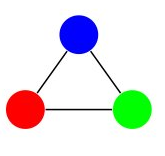
\includegraphics[scale=0.77]{3colouring.png}
\end{center}

The output of the decision would be whether or not the graph $\emph{G}$ admits a proper vertex colouring with $\emph{k}$ colours. There is also a special case where a graph is 2 colourable and can be be done in $\emph{P}$ (Polynomial-time) and this is were the particular graph that we're colouring is bipartite which is a particular graph whose vertices can be divided into two disjoint sets were every edge that connects a vertex in $\emph{U}$ to one in $\emph{V}$.



\vspace{3mm}
The next step with graph colouring would be the optimisation which the chromatic number. The chromatic number refers to the smallest number of colours needed to colour a graph $\emph{G}$ is called the chromatic number and is often denoted by $\emph{X}$($\emph{G}$). With the optimisation process we will have an input of a graph $\emph{G}$ with $\emph{n}$ vertices. We will firstly have a look at the simplest form which is not bipartite. We have looked at this previously which is the triangle $\emph{K}$$^{3}$.

\vspace{3mm}
The first example that I will show is that a complete graph $\emph{K}$$^{3}$ with $\emph{n}$ vertices is $\emph{n}$-colourable but not (n-1) colourable. This is shown below showing that $\emph{K}$$^{3}$ is not 2 colourable. Another rule we would have to follow would be that $\emph{K}$$_{n}$ has a vertex set $\lbrace$1,...,n$\rbrace$ and all possible $\frac{1}{2}$ $\emph{n}$ ($\emph{n}$-1) edges. I will look at another example to prove the chromatic number which will be the graph $\emph{K}$$_{4}$ with 4 vertices is 4 colourable as shown below:

\begin{center}
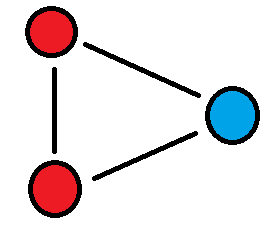
\includegraphics[scale=0.60]{not3colouring.png}
\end{center}

\vspace{3mm}

\begin{center}
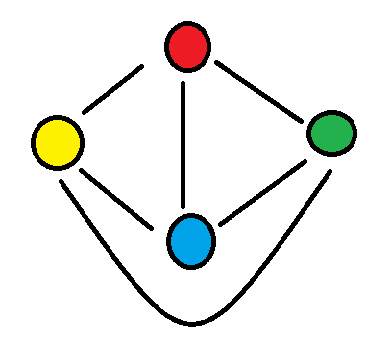
\includegraphics[scale=0.60]{4colouring.png}
\end{center}

\vspace{3mm}
On the other hand the same graph will not be $\emph{n}$-1 colourable (4-1 = 3 colourable). The graph above proves it's not 3 colourable as well as showig the graphs has the correct number of edges for a $\emph{K}$$_{4}$ graph. $\frac{1}{2}$ $\emph{n}$ ($\emph{n}$-1) edges = 2(3) = 6.

\vspace{3mm}

The graph colouring problem is to determine the minimum number of colours needed to colour a given undirected graph. To prove that the 3 colouring graph problem is NP-complete we use a reduction from 3SAT. The smallest case is $\emph{K}$$^{3}$. 

\begin{proof}
The set $\emph{V}$ consists of a vertex for each variable, a vertex for the negation of each variable, 5 vertices for each clause and 3 special vertices: True, False and Red. The edges of the graph are of two types: "literal" edges that are independentof the clauses and "clause" edges that depend on the clauses. The literals edges from trianle on the special vertices and also form a triangle on $\emph{X}$$_{i}$, $\neg$$\emph{X}$$_{i}$ and RED for $\emph{i}$ = 1, 2, ..., $\emph{n}$. [1] 
\end{proof}

\begin{center}
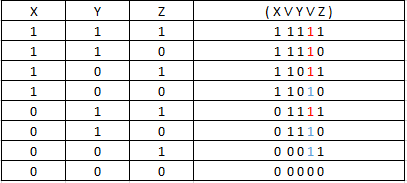
\includegraphics[scale=0.60]{truthtable2.png}
\end{center}

The truth table above shows for $\emph{K}$$_{3}$ can be reduced to 3CNF with the following clause ( X $\bigvee$ Y $\bigvee$ Z), if and only if one of the variables X, Y or Z is coloured true. If each of x, y and z is coloured True or False, then the graph is only 3 colourable if and only if at least one of the variables x, y or z is coloured True. The graph below illustrates this for the case when $<$ X = 1, Y = 0 and Z = 0 $>$:

\begin{center}
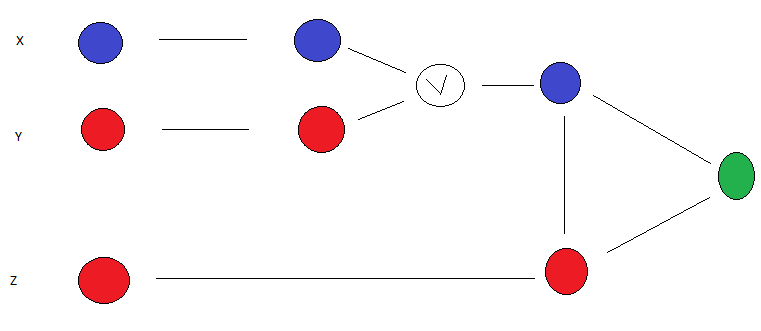
\includegraphics[scale=0.60]{graph1.png}
\end{center}

There is no legal 3-colouring of the above graph in which x, y and z are all coloured False but if any x, y, z are coloured True then there is a legal 3-colouring of the above graph.
\subsection{SAT}

\begin{defi}
An instance of SAT is a Boolean formula composed of $\emph{n}$ Boolean variables such as $\emph{X}$$_{1}$,$\emph{X}$$_{2}$,..., $\emph{X}$$_{n}$; and $\emph{m}$ Boolean connectives any Boolean function with one or two inputs and one output, such as $\bigwedge$ (AND), $\bigvee$ (OR), $\neg$ (NOT), $\rightarrow$ (implication), $\leftrightarrow$ (if and only if); and Parentheses (Without loss of generality, we assume that there are no redundant parentheses, i.e. there is at mose one pair of parentheses per Boolean connective).
\end{defi}

As an example, I will show it with the following formula:

$\phi$ = (($\emph{x}$$_{1}$ $\rightarrow$ $\emph{x}$$_{2}$) $\bigvee$ $\neg$ (($\emph{x}$$_{1}$ $\leftrightarrow$ $\emph{x}$$_{3}$) $\bigvee$ $\emph{x}$$_{4}$)) $\bigwedge$ $\neg$ $\emph{x}$$_{4}$


Has the satisfying assignment $<$$\emph{x}$$_{1}$ = 0, $\emph{x}$$_{2}$ = 0, $\emph{x}$$_{3}$ = 1 and $\emph{x}$$_{4}$ = 1$>$

= ((0 $\rightarrow$ 0) $\bigvee$ $\neg$(($\neg$0 $\leftrightarrow$ 1) $\bigvee$ 1)) $\bigwedge$ $\neg$0

= (1 $\bigvee$ $\neg$(1 $\bigvee$ 1)) $\bigwedge$ 1

= (1 $\bigvee$ 0) $\bigwedge$ 1

= 1


This shows that the following formula $\phi$ belongs to SAT [1].

\vspace{3mm}
The SAT problem is $\emph{P}$ when the number of literals in each clause is limited to two. The name given to this kind problem is 2SAT. As long as there are two literals in each clause the 2SAT problem can be solved in polynomial time.

\vspace{3mm}
The 3SAT is an extenstion of the SATISFIABILITY problem, where each clause must contain exactly 3 literals. The properties of 3SAT are as follow:

\begin{defi}
We transform SAT to 3SAT. Let $\lbrace$$u_{1}$,u$_{2}$,...,u$_{n}$$\rbrace$ be a set of variables and $\emph{C}$ = $\lbrace$c$_{1}$,c$_{2}$,...,c$_{n}$$\rbrace$ be a set of clauses making up an arbitrary instance of SAT. We shall construct a collection of $\emph{C'}$ of three-literal clauses on a set $\emph{U'}$ of variables such that $\emph{C'}$ is SATISFIABLE if and only if $\emph{C}$ is SATISFIABLE. [2]
\end{defi}

Here is an example of a 3SAT Boolean logic in Conjunctive Normal Form;

$\phi$ = ($\neg$$\emph{x}$$_{1}$ $\bigvee$ $\neg$$\emph{x}$$_{2}$ $\bigvee$ $\emph{x}$$_{3}$) $\bigwedge$ ($\emph{x}$$_{1}$ $\bigvee$ $\emph{x}$$_{2}$ $\bigvee$ $\emph{x}$$_{3}$)

\vspace{2mm}
With the example 3SAT Boolean formula I have given above, the truth table below shows that the answer to this instance is YES.

\begin{center}
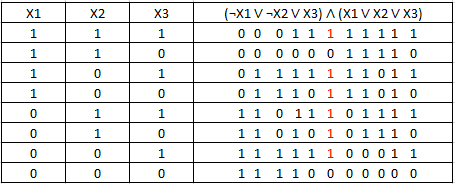
\includegraphics[scale=0.60]{truthtable.png}
\end{center}

I have solved the instance of the decision with a truth table where there is a truth value. Firstly we assign a True and False value to each of the variables for all the different cases, which would be 2$^{n}$ in this particular case it would be 2$^{3}$. In this particular Boolean logic instance, there is the case where $<$X1 = 1, X2 = 1 and x3 = 1 $>$

\vspace{3mm}
Assuming that we are given a formula in Conjunctive Normal Form which has three distinct literals, the reduction algorithm gives us an instance of the SUBSET-SUM problem which is only SATISFIABLE if and only if there is a subset of $\emph{S}$ whose sum  is exactly $\emph{T}$.

\vspace{3mm}
First, no clause contains both variable and its negation, for such that a clause is automatically satisfied by any assignment of values the variables. Second, each variable appears in at least one clause, for otherwise it does not matter what value is assigned to the variables. [1]

\vspace{3mm}
The following table below shows an example of the SUBSET-SUM with a set $\emph{S}$ and a target $\emph{T}$ with the formula in 3-CNF being: C1 AND C2 AND C3 AND C4 where C1 = ( X1 $\bigvee$ $\neg$X2 $\bigvee$ $\neg$X3 ) C2 = ( $\neg$X1 $\bigvee$ $\neg$X2 $\bigvee$ $\neg$X3) C3 = ( $\neg$X1 $\bigvee$ $\neg$X2 $\bigvee$ X3 ) and C4 = ( X1 $\bigvee$ X2 $\bigvee$ X3 ).

\begin{center}
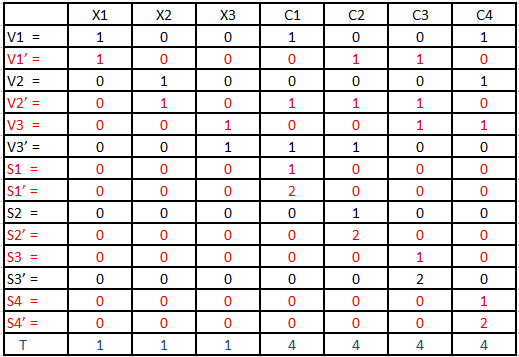
\includegraphics[scale=0.60]{subset.png}
\end{center}

The target has a 1 in each digit variable and a 4 in each digit labelled by a clause for each variable $\emph{X}$$_{i}$, there are two integers, $\emph{V}$$\emph{i}$ and $\emph{V}$$_{i}$' in S. Each has a 1 in the digit labelled $\emph{X}$$_{i}$ and 0's in the other variable digits. If literal $\emph{X}$$_{i}$ appears in clause $\emph{C}$$_{i}$, then the digit labelled by $\emph{C}$$_{i}$ in $\emph{V}$$_{i}$ contains 1. If literal $\neg$$\emph{X}$$_{i}$ appears in clause $\emph{C}$$_{i}$, then the digit labelled by $\emph{C}$ in $\emph{V}$$_{i}$' contains a 1. All other digits labelled by clauses in $\emph{v}$$_{i}$ and $\emph{v}$$_{i}$' are 0. All $\emph{v}$$_{i}$ and $\emph{v}$$_{i}$' values in the set $\emph{S}$ are unique. Why? for $\emph{I}$ $\neq$ $\emph{i}$, no $\emph{V}$$_{i}$ or $\emph{V}$$_{i}$' values can equal $\emph{V}$$_{i}$ and $\emph{V}$$_{i}$' in the most significant $\emph{n}$ digits. [1]

\vspace{3mm}
$\emph{S}$ = $\lbrace$1001001, 1000110, 101110, 10011, 11100, 2000, 100, 200, 10, 1, 2$\rbrace$. Our target is $\emph{T}$. The subset $\emph{S'}$ $\subseteq$ $\emph{S}$ contains $\emph{V1}$, $\emph{V2}$ and $\emph{V3}$. It also contains slack variables $\emph{S1}$, $\emph{S2'}$, $\emph{S3}$, $\emph{S4}$ and $\emph{S4'}$ to achieve our target value 114444.

\vspace{3mm}



\begin{proof}
Here is my proofjkb  
\end{proof}

\subsection{Hamiltonian Problem}
The Hamiltonian problem in mathematical field of graph theory are of the following two types. The Hamiltonian path problem and the Hamiltonian cycle which are problems of determining whether a given Hamiltonian path or a Hamiltonian cycle exists in a given graph. The Hamiltonian path problem and the Hamiltonian cycle problem are both NP-complete. 


\begin{defi}
Given a graph $\emph{G}$ = (V,E) our certificate is the sequence of $\vert$V$\vert$ vertices that make up the Hamiltonian cycle. The verification algorithm checks that this sequence contains each vertex in $\emph{V}$ exactly once and that with the first vertex repeated at the end, it forms a cycle $\emph{G}$. That is, it checks that there is and edge between each pair of consecutive vertices and between the first and the last vertices. This verification can be performed in polynomial time. [1]
\end{defi}

\vspace{3mm}

The trivial graph on a single node is said to be a Hamiltonian cycle, but the connected graph on two nodes is not. The dodecahedron is also Hamiltonian but it's not the case that all graphs are Hamiltonian, for example a bipartite graph with odd number vertices is not Hamiltonian as shown below; 


\begin{center}
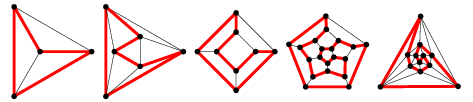
\includegraphics[scale=0.80]{Hamiltonian1.png}
\end{center}

\begin{center}
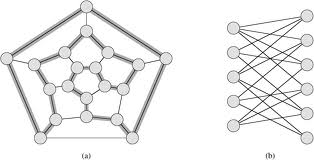
\includegraphics[scale=0.75]{bipartite.png}
\end{center}

\vspace{3mm}
I will now go onto show that the Hamiltonian cycle problem is NP-complete as I will reduce the Hamiltonian problem from Vertex-cover. The following construction will be based on a widget, which is a piece of a graph that enforces certain properties.

\vspace{3mm}
For each edge (u,v) $\in$ $\emph{E}$, the graph $\emph{G'}$ that we construct will contain one copy of the widget, which we denote by $\emph{W}$$_{u,v}$. We denote each vertex in $\emph{W}$ by [u,v,i] or [v,u,i] where 1 $\leq$ i $\leq$ 6, so that each widget $\emph{W}$$_{u,v}$ contains 12 vertices. [1]

\vspace{3mm}

One of the properties that will be enforced by the widget is that only vertices to have edges incident from the outside are the following [u,v,1], [u,v,6], [v,u,1], and [v,u,6]. If the cycle was to enter through [u,v,1] it would have to exist through [u,v,6].

\vspace{3mm}
The only other vertices in $\emph{V'}$ other than those of widgets are selector vertices $_{s1}$,$_{s2}$,...,$_{sk}$. We use edges incident on selector vertices in $\emph{G'}$. First, for each vertex $\emph{u}$ $\in$ $\emph{V}$, we add edges to join pairs of widgets in order to form a path containing all widgets corresponding to edges incident on $\emph{u}$ in $\emph{G}$. We arbitrarily order of vertices adjacent to each vertex $\emph{u}$ $\in$ $\emph{V}$ as $\emph{u}$$^{(1)}$, $\emph{u}$$^{(2)}$,...,$\emph{u}$$^{(degree(u))}$, where degree($\emph{u}$) is the number of vertices adjacent to $\emph{u}$. We create a path in $\emph{G'}$ through all the widgets corresponding to eges incident on $\emph{u}$ by addingto $\emph{E'}$ the edges $\lbrace$([u,u$^{i}$,6], [u,u$^{(i+1)}$,1] : 1 $\leq$ i $\leq$ degree($\emph{u}$) - 1$\rbrace$. [1]

\begin{center}
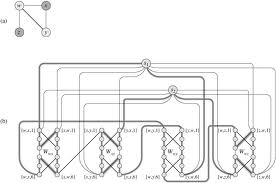
\includegraphics[scale=0.85]{download.png}
\end{center}

\subsection{Vertex Cover }
In mathematical discipline of graph theory, a vertex cover of a graph is a set of vertices such that each edge of the graph is incident to at least one vertex.

\begin{defi}
A vertex cover of an undirected graph $\emph{G}$ = ($\emph{V,E}$) is a subset $\emph{V'}$ $\subseteq$ $\emph{V}$ such that if (u,v) $\in$ $\emph{E}$, then $\emph{u}$ $\in$ $\emph{V'}$ or $\emph{v}$ $\in$ (or both). That is, each vertex "covers" its incident edges, and a vertex cover for $\emph{G}$ is a set of vertices that covers all edges in $\emph{E}$. The size of vertex cover is the number of vertices in it. [1]
\end{defi}

\begin{center}
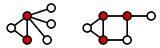
\includegraphics[scale=1.11]{vertex1.png}
\end{center}

We first show that vertex-cover $\in$ NP. Suppose we are given a graph $\emph{G}$ = ($\emph{V,E}$) and an integer $\emph{k}$. The certificate we choose is the vertex cover $\emph{V'}$ $\subseteq$ $\emph{V}$ itself. The verification algorithm affirms that $\vert$V$\vert$ = k, and then it checks, for each edge (u,v) $\in$ $\emph{V'}$ or v $\in$ $\emph{V'}$. This verifivation can be performed straight forwardly in polynomial time. [1]

\begin{center}
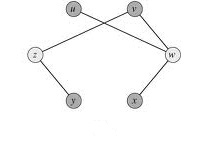
\includegraphics[scale=0.90]{vertex.png}
\end{center}

The reduction is based on the notion of the complement of a graph so I will reduce vertex cover from another NP-complete problem which is based on graph theory. In this case I will reduce the vertex-cover problem from clique.

\vspace{3mm}
Given an undirected graph $\emph{G}$ = (V,E), we define the complement of $\emph{G}$ as $\emph{G}$ = $\lbrace$(V,E), where $\emph{E}$ = $\lbrace$(u,v):u,v $\in$ $\emph{V}$, and (u,v) $\not$$\in$ $\emph{E}$$\rbrace$. In other words, $\emph{G}$ is the graph containing exactly those edges that are not in $\emph{G}$. [1]


\begin{center}
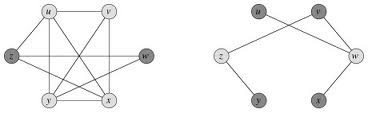
\includegraphics[scale=0.70]{vertex3.png}
\end{center}

\vspace{3mm}
The first image has a clique $\emph{V'}$ which is of size 4, clique $\emph{V'}$ = $\lbrace$u,v,x,y$\rbrace$. What we then do is create a second graph containing exactly those edges that are not in the previous graph. The vertex covers are the vertices which are in the clique set. Those which are not in the clique set are the vertices, which the cover-vertex are incident to.

\vspace{3mm}
The reduction algorithm takes as input an instance $\langle$G,K$\rangle$ of the clique problem. It computes the complement $\emph{G}$, which is easily done in polynomial time. The output of the reduction algorithm is the instance $\langle$$\emph{G}$,$\vert$V$\vert$ - K$\rangle$ of the vertex cover problem. The graph $\emph{G}$ has a clique of size $\emph{k}$ if and only if the graph $\emph{G}$ has a vertex cover of size $\vert$V$\vert$-K.[1]

\vspace{3mm}
In our reduction example this holds as we a have a graph $\emph{G}$ which has a vertex cover of size $\vert$V$\vert$ which is the number of vertices the graph has. In our example it is 6 - k which k has was the number of cliques, 4 so in in our example we would have a vertex cover which is 2.

\vspace{3mm}
Graph $\emph{G}$ has a clique $\emph{V'}$ $\subseteq$ $\emph{V}$ with $\vert$V'$\vert$ = K. So in our example we have the following vertices $\lbrace$u,v,y,x,z,w$\rbrace$. The following statement holds as $\lbrace$u,v,y,x$\rbrace$ $\subseteq$ $\lbrace$w,z,v,u,x,y$\rbrace$.

\vspace{3mm}
Another statement thats holds is that Let (u,v) be any edge $\emph{E}$. Then (u,v) $\not\in$ $\emph{E}$,which implies that at least one of the $\emph{u}$ or $\emph{v}$ do not beling to $\emph{V'}$.

\vspace{3mm}
For the following clique $\lbrace$u,v,y$\rbrace$. The $\emph{V}$ vertex uses all its edges as does the $\emph{Y}$ vertex but the $\emph{U}$ vertex only uses one of the edges.



\subsection{Clique}
The clique problem refers to any of the problems related to finding particular complete subg-graphs, which are sets of elements where each pair of element is connected. The clique decision problem include the following, finding the maximum clique, which is a clique with the largest number of vertices. Also, finding the maximum weight clique in a weighted graph. Thirdly, listing all maximal cliques, which are cliques that cannot be enlarged. Finally, determining the decision problem which is testing whether a graph contains a clique larger than a given size.

\begin{defi}
The clique is an undirected graph $\emph{G}$ = (V,E) is a subset $\emph{V'}$ $\subseteq$ $\emph{V}$ of vertices, each pair of which is connected by an edge in $\emph{E}$. In other words, a clique is a complete subgraph of $\emph{G}$. The size of a clique is the number of vertices it contains. The clique problem is the optimization problem finding a clique of maximum size in a graph. As a decsion problem, we ask simply whether a clique of a given size $\emph{k}$ exists in the graph. The formal definitions is 

CLIQUE = $\lbrace$$\langle$G,K$\rangle$ : G is a graph with a clique of size k $\rbrace$
\end{defi}

\begin{center}
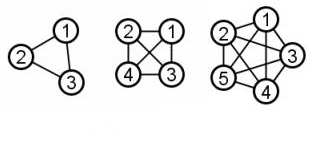
\includegraphics[scale=0.80]{clique.png}
\end{center}


\vspace{3mm}
A naive algorithm for determining whether a graph $\emph{G}$ = (V,E) with $\vert$V$\vert$ vertices has a clique of size $\emph{k}$ is to list all $\emph{k}$ subsets of $\emph{V}$, and check each one to see whether it forms a clique. The running time of this algorithm if polynimial if $\emph{k}$ is a constant. To show that CLIQUE $\in$ NP, for a given graph G = (V,E),we use the set $\emph{V'}$ $\subseteq$ $\emph{V}$ of vertices in the clique as a certificate for $\emph{G}$. Checking whether, for each pair u,v $\in$ $\emph{V'}$\, the edge (u,v) belongs to $\emph{E}$. [1]

The following redcution will show that the clique decision problem is in NP-complte. We start the reduction with an instance of 3SAT an example wpuld be as follows:

\vspace{3mm}
$\phi$ = (x$_{1}$ $\bigvee$ x$_{2}$ $\bigvee$ x$_{3}$) $\bigwedge$ (x$_{1}$ $\bigvee$ x$_{2}$ $\bigvee$ x$_{3}$) $\bigwedge$ (x$_{1}$ $\bigvee$ x$_{2}$ $\bigvee$ x$_{3}$)

\vspace{3mm}
The following example shows a Boolean formula of 3 conjunctive normal form which has three clauses. A 3 conjunctive normal form formula can have as many k clauses but each clause must have exactly the distinct literals $\emph{L}$$_{1}$, $\emph{L}$$_{2}$ and $\emph{L}$$_{3}$.

\vspace{3mm}
I will now go onto show a graph $\emph{G}$ so that the 3CNF formula is SATISFIABLE if and only if $\emph{G}$ has a clique of size $\emph{k}$.

\vspace{3mm}
The graph $\emph{G}$ so (V,E) is constructed as follows. For each clause $\emph{C}$$^{r}$ = (L$_{1}$ $\bigvee$ L$_{2}$ $\bigvee$ L$_{3}$) in $\phi$, we place a triple of vertices $\emph{v1}$, $\emph{v2}$ and $\emph{v3}$ into $\emph{V}$. We put an edge between two vertices $\emph{v}$$_{i}$$^{r}$ and $\emph{v}$$_{j}$$^{s}$ if both of the following hold:

\begin{itemize}
\item
$\emph{v}$$_{i}$$^{r}$ and $\emph{v}$$_{j}$$^{s}$ are in different triple, that is r $\ne$ s, and 

\item
their coresponding literals are consistent, that is, $\emph{v}$$_{i}$$^{r}$ is not the negation of $\emph{v}$$_{j}$$^{s}$ [1]

\end{itemize} 

This graph can be easily computed from a given $\phi$ in polynomial time. I will shows this as an example below given the following formula;

\vspace{3mm}
$\phi$ = (x1 $\bigvee$ $\neg$x2 $\bigvee$ $\neg$x3) $\bigwedge$ ($\neg$x1 $\bigvee$ x2 $\bigvee$ x3) $\bigwedge$ (x1 $\bigvee$ x2 $\bigvee$ x3)

\vspace{3mm}
The satisfying assignment of the formula has x2 = 0, x3 = 1 and x1 may be either 0 or 1 (where 1 is true and 0 is false). This would satisfy where c1 with $\neg$x2, and it satisfies c2 and c3 with x3. This constructs a clique which is of size 3 as shown below;

\begin{center}
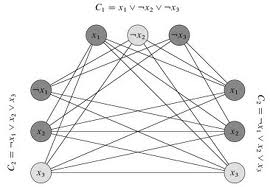
\includegraphics[scale=0.60]{clique1.png}
\end{center}

We claim that $\emph{V'}$ is a clique. For any two vertices $\emph{v}$$_{i}$$^{r}$, $\emph{v}$$_{j}$$^{s}$, where r $\neq$ s, both corresponding literals $\emph{L}$$_{i}$$^{r}$, $\emph{L}$$_{j}$$^{s}$ are mapped to 1 by the given satisfying assignment and thus, by the construction of $\emph{G}$, the edge ($\emph{v}$$_{i}$$^{r}$,$\emph{v}$$_{j}$$^{s}$) belongs to $\emph{E}$. No edges in $\emph{G}$ connect vertices in the same triple, and so $\emph{V'}$ contains exactly one vertex per triple. Since $\emph{G}$ contains no edges between inconsistent literals each clause is satisfied, and so $\phi$ is satisfied. [1]

\subsection{Sudoku}

\begin{defi}
A problem is given as a n$^{2}$ x n$^{2}$ grid which is divided into n x n subgrids. The value n is called order since the cells are filled with an integer from 1 through n$^{2}$ and the goal is to fill in all the blank cells so that each row, column and n x n subgrid has each of the integers from 1 through n$^{2}$ exactly once.

\end{defi}

\begin{center}
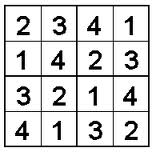
\includegraphics[scale=0.60]{sudoku.png}
\end{center}

\vspace{3mm}
Sudokou is often represented by a 9 x 9 grid which consists of 3 x 3 subgrids. Some of the boxes are filled with numbers from 1 to 9,there are also blanks that need to be filled such that every row, every column and every 3 x 3 subgrid contains each of the 9 posible numbers.

\begin{center}
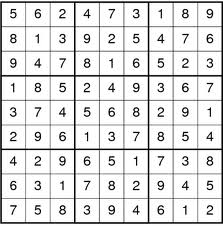
\includegraphics[scale=0.60]{9x9sud.png}
\end{center}

I will only discuss sudoku puzzles that have the following properties;

\begin{enumerate}
\item
Sudoku puzzles that have only one solution
\item
Sudoku puzzles that can be solved with only reasoning 
\end{enumerate}

The following reduction will show that given a Latin square $\emph{L}$ were every row and column contains each of the n possible numbers can be trasnformed into Sudoku were every row, column and subgrid contains each of the n possible numbers.

\vspace{3mm}
In the argument below, we use integers ranged from 0(instead of 1) as row and column numbers and contents of cells, and write $\emph{S}$(i,j) for entry at position (i,j) of square $\emph{S}$ ($\perp$ means a blank).[6]

\vspace{3mm}

\begin{center}
$\emph{Lemma}$ Let $\emph{S}$ be a Number Place of order n such that 


$\emph{S}$(i,j) = $\perp$ (whene(i,j) $\in$ $\emph{B}$)

((i mod n)n + $\lfloor$$\frac{i}{n}$$\rfloor$ + j) mode n$^{2}$ (otherwise)

where $\emph{B}$ = $\lbrace$(i,j) $\vert$ $\lfloor$$\frac{i}{n}$$\rfloor$ = 0 and (j mode n) = 0$\rbrace$. Then a square $\emph{S'}$ obtained by filling in the blanks of $\emph{S}$ is a solution to $\emph{S}$ if and only if 
\end{center}
\begin{itemize}
\item
For any (i,j) $\in$ $\emph{B}$, $\emph{S'}$(i,j) mod n equals 0.
\item
A square $\emph{L}$ defined by $\emph{L}$(i,j/n) = $\emph{S'}$(i,j)/n for all (i,j) $\in$ $\emph{B}$ is a Latin.[6]
\end{itemize}

\end{document}